\documentclass{book}

\usepackage[utf8]{inputenc}
\usepackage{natbib}
\usepackage{listings}
\usepackage{amsmath}
\usepackage{pdfpages}
\usepackage{xcolor}
\usepackage{listings}
\usepackage{color}
 
\renewcommand{\lstlistingname}{Code} 
 
\definecolor{dkgreen}{rgb}{0,0.6,0}
\definecolor{gray}{rgb}{0.5,0.5,0.5}
\definecolor{mauve}{rgb}{0.58,0,0.82}

\lstset{frame=tb,
  language=bash,
  aboveskip=3mm,
  belowskip=3mm,
  showstringspaces=false,
  columns=flexible,
  basicstyle={\small\ttfamily},
  numbers=none,
  numberstyle=\tiny\color{gray},
  keywordstyle=\color{blue},
  stringstyle=\color{mauve},
  breaklines=true,
  breakatwhitespace=true,
  tabsize=3
}

\title{Motoman manual}
\author{Thibault Barbié}
\date{\today}


\begin{document}
\begin{titlepage}
\newcommand{\HRule}{\rule{\linewidth}{0.5mm}}
\center

\HRule \\[1.5cm]
{ \huge \bfseries Motoman manual}\\[0.4cm] 
\HRule \\[1.5cm]

\begin{minipage}{0.4\textwidth}
\begin{flushleft} \large
\emph{Author:}\\
Thibault \textsc{Barbi\'{e}} % Your name
\end{flushleft}
\end{minipage}
~
\begin{minipage}{0.4\textwidth}
\begin{flushright} \large
\emph{Version:}\\
0.0.1 % Your name
\end{flushright}
\end{minipage}\\[4cm]

{\large \today}\\[3cm] 
\vfill 

\end{titlepage}

\tableofcontents
\newpage

\section{Introduction}

The motoman industrial robot is a complicated system that needs to be handled carefully. This manual was written to help to understand how to do basic operations such as connecting the robot to its rviz visualization, using motion planners and using the kinects.

The motoman robot is a very expensive system, if you are scared to do something wrong that could break it then please ask the more experienced lab members.
\chapter{Installation and first script}

In this chapter we will explain how to install the motoman project on your computer and make you write a script that use a motion planner to find a plan for the robot. This chapter is essentially a chain of instructions, there are few details about the files you will manipulate. The next chapter will be more in depth.

\section{Initialization}
First thing to do is to create a ROS workspace where you will work.  So go to where you want to create your workspace and then create the workspace with a \emph{src} folder inside. Then go inside the \emph{src} folder and initialize the catkin workspace.

\begin{lstlisting}
cd /where/you/want/your/workspace
mkdir -p my_workspace/src
cd my_workspace/src
catkin_init_workspace
\end{lstlisting}

Then download the motoman project repository. To do it you need to have the git software in your computer. To install git just type the following command.

\begin{lstlisting}
sudo apt-get install git
\end{lstlisting}

Then you need to download the repository. The \emph{clone} command after the \emph{git} command means you want to take the repository data and copy them into your current folder. So first go where your ros workspace and clone the github repository inside the \emph{src} folder.  

\begin{lstlisting}
cd my_workspace/src
git clone https://github.com/Nishida-Lab/motoman_project.git
\end{lstlisting}

Then normaly a \emph{motoman\_project} file would have been created in your \emph{src} folder. The next step is to actually compile the project. To do this you need to use the \emph{catkin\_make} command in the root of your workspace. But before that you need to be sure to have all the dependencies. 


\begin{lstlisting}
cd my_workspace
wstool init src src/motoman_project/dependencies.rosinstall
sudo apt-get install ros-indigo-industrial-msgs
sudo apt-get install ros-indigo-industrial-robot-simulator
sudo apt-get install ros-indigo-industrial-robot-client
sudo apt-get install ros-indigo-ros-controllers
rosdep install -i --from-paths src
catkin_make
\end{lstlisting}

After compiling everything (it could take some time!) you will be able to use the project. A simple test is to launch one of the launch file of the project. First you need to source the workspace to be sure that you can use the ROS command associated to your project.

\begin{lstlisting}
cd workspace
source devel/setup.bash
\end{lstlisting}

Then launch the empty environment with motoman inside by the following command.

\begin{lstlisting}
cd my_workspace
source devel/setup.bash
roslaunch motoman_gazebo sia5_empty_world.launch
\end{lstlisting}
\begin{figure}
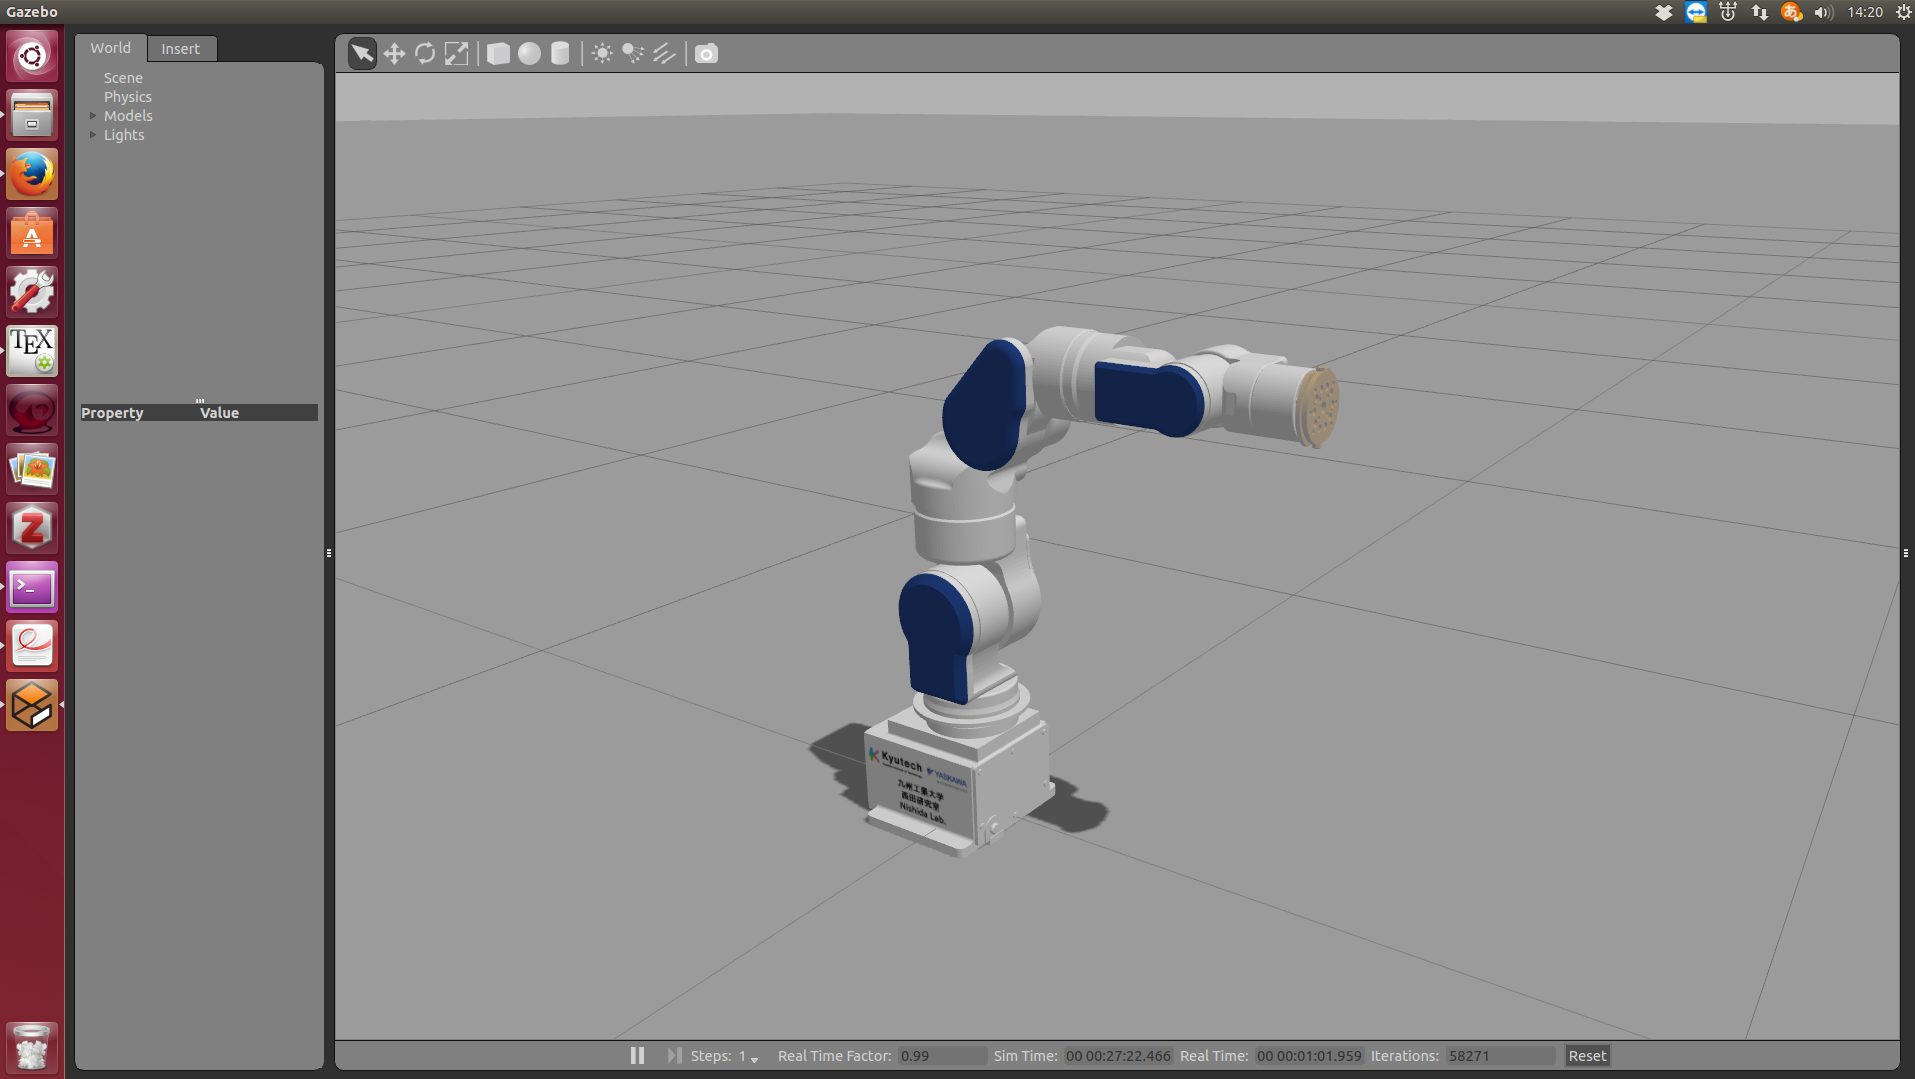
\includegraphics[scale=0.132]{images/installation_first/launch_gazebo.png}
\centering
\caption{That is what you should see if the installation has been rightly completed.}
\label{fig:launch_gazebo}
\end{figure}
You should normally have the gazebo software begin to run and you can soon see the motoman robot sia5 inside your screen like in Figure \ref{fig:launch_gazebo}.

\section{Finding a motion plan}

In this section we will create a script that connect to the robot and use a motion planner to find a plan between a start position and a goal position. There are many things to do before being able to do it but if you follow the steps it should not be difficult. This section focus on writing the script rather than understanding everything. The next chapters will give more details about it.

To begin everything we need to create a ros package where our script will be written. You normally have one metapackage in your \emph{src} folder named \emph{motoman\_project}. It is really easy to create a new package in ros with the catkin command. You can name it anything you want, in this manual we will call it \emph{motion\_planning}. To make our script able to run we will need to initialize gazebo and rviz. For this reason you will need to launch gazebo and rviz every time you will want to use your script. As it is tiring it is easier to just create a launch file that will be launch before the script and that will automatically call the gazebo and rviz part by itself.


\begin{lstlisting}
cd workspace/src
catkin_create_pkg motion_planning roscpp
cd motion_planning
mkdir launch
cd launch
touch initialization.launch
\end{lstlisting}

We use the \emph{roscpp} argument because our package will need it to create a ros node. You can create the following launch file in the launch folder, we will describe it more later. 

\lstinputlisting[caption=initialization.launch]{code_files/installation_first/initialization.launch}


In the \emph{src} folder we can write our script to move the robot. First we create the file (we named it \emph{moving.cpp} but every name is ok, just change the CMakeLists file accordingly). 

\begin{lstlisting}
cd workspace/src/motion_planning/src
touch moving.cpp
\end{lstlisting}

Then just write the following code inside the \emph{moving.cpp} file. This script shows how to ask moveit to find a plan from the current position to any goal position you define. However it may be possible that no plan will be found. In this situation the workspace is empty so it should be quite easy to find a solution but when a lot of obstacles are populating the environment then it becomes a difficult task to find a collision free trajectory for the robot.

\lstinputlisting[language=c++,caption=moving.cpp]{code_files/installation_first/moving.cpp}

After having wrote the script we need to compile it. To do it we need to modify two files : the CMakeLists.txt and package.xml. These two files have already been created when you created the package with the catkin command, so you just have to replace their contents with the following files.

\lstinputlisting[caption=CMakeLists.txt]{code_files/installation_first/CMakeLists.txt}

\lstinputlisting[caption=package.xml]{code_files/installation_first/package.xml}


So now everything have been done to use the script you wrote. First compile everything. Every time you will modify your C++ files you will need to compile again all your workspace. Once compile you will need to first launch the launch file that will initialize gazebo and rviz, it will also load the ompl library. When the launch file has been ran you can then run your script.


\begin{lstlisting}
cd workspace
catkin_make
source devel/setup.bash
roslaunch motion_planning initialization.launch
rosrun motion_planning motion_planning
\end{lstlisting}


The result of this script could be seen in Figure \ref{fig:simple_moving}. The figure shows a trail of the movement. You can activate it by clicking on the left panel to the \emph{motion planning} line and then clicking on the \emph{Show trail} box as it can be seen in the Figure \ref{fig:show_trail}.  

\begin{figure}
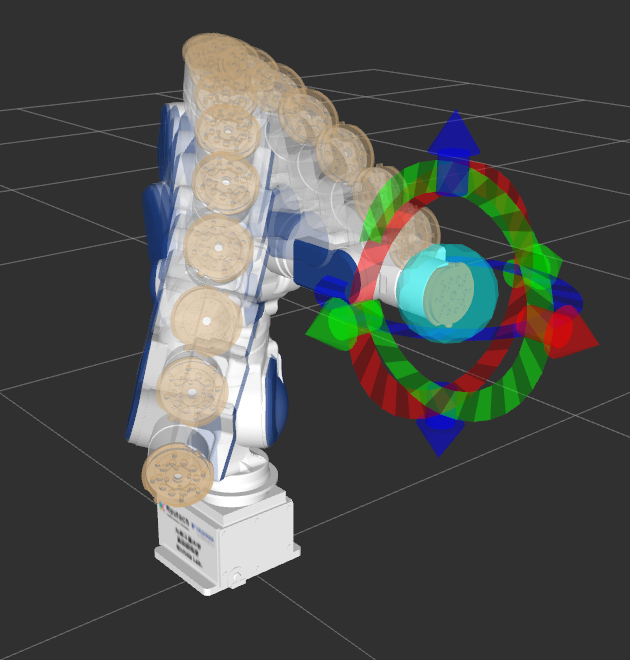
\includegraphics[width=8cm]{images/installation_first/simple_moving.png}
\centering
\caption{Yo}
\label{fig:simple_moving}
\end{figure}



\begin{figure}
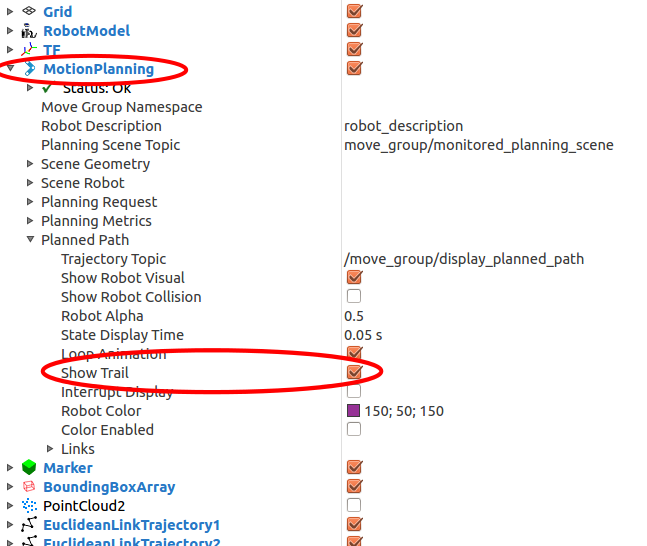
\includegraphics[width=8cm]{images/installation_first/show_trail.png}
\centering
\caption{Yo}
\label{fig:show_trail}
\end{figure}
\chapter{Motion planning}

This chapter will focus on the motion planning part. You will learn how to select the motion planner you want (RRT, RRT*, STOMP, CHOMP...), how to create a planning problem and how to solve it.

\section{GUI utilisation}

We can directly use the GUI to solve some motion planning problems. Indeed, moveit has an interface in rviz. Using the GUI will be usefull when you want to quickly test your robot motion or a planning problem. It can also show how long it will last for the motion planner you selected to find a motion plan. However, when you will need to find precise plan (with exact coordinate for joints) or when you will want to generate a lot of trajectories it will be far easier to use scripts.

Using the GUI is really simple. First go to the \emph{motion planning} tab and click on the \emph{planning} tab after (figure \ref{fig:gui_procedure_1}). In this tab you can select your start state and your goal state. Initially the start state should be initialized with the current position of your robot which should be its home position. However, if it not the case you can initialize it yourself by clicking on the \emph{select start state} tab and clicking on the \emph{update} button (the current option should be selected) as shown in figure \ref{fig:gui_procedure_2}. You can see that you can choose other ways to initialize the start goal. For instance you can decide to select a random valid position or pre-determined position. The pre-determined position are generated with the moveit initialization procedure. If you use the motoman project it should have only two pre-determined position : the home position and the up position. As for the goal position, you can either do the same as the start position (selecting random position or pre-determined ones) or just use your mouse and move the robot through the light blue ball inside the gui (see figure \ref{fig:gui_end_effector}).
\begin{figure}
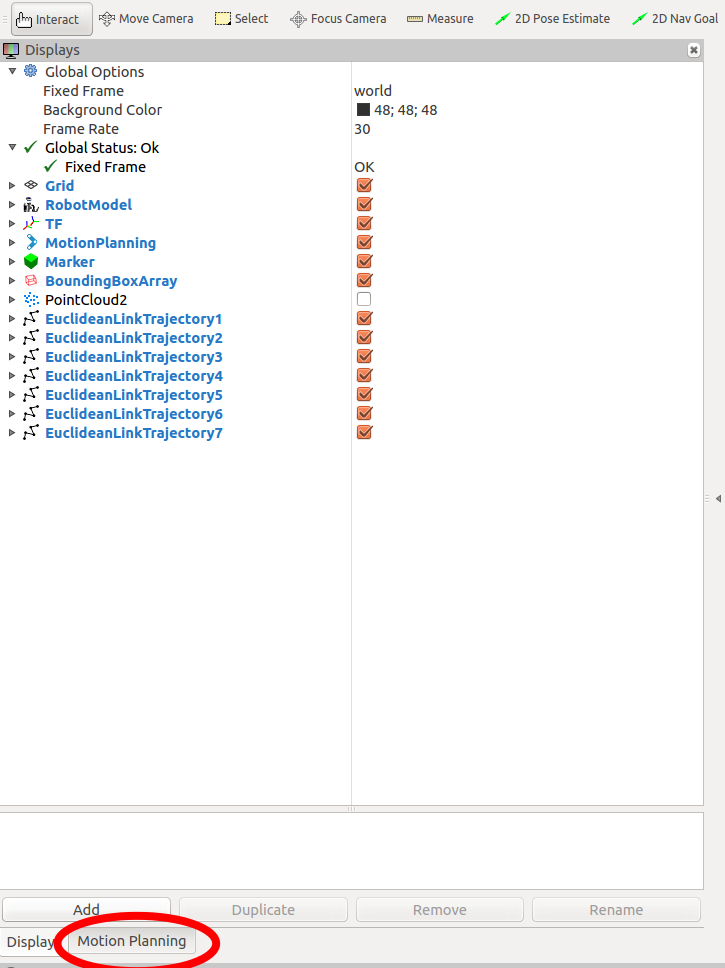
\includegraphics[scale=0.23]{images/motion_planning/gui_moving_procedure_1.png}
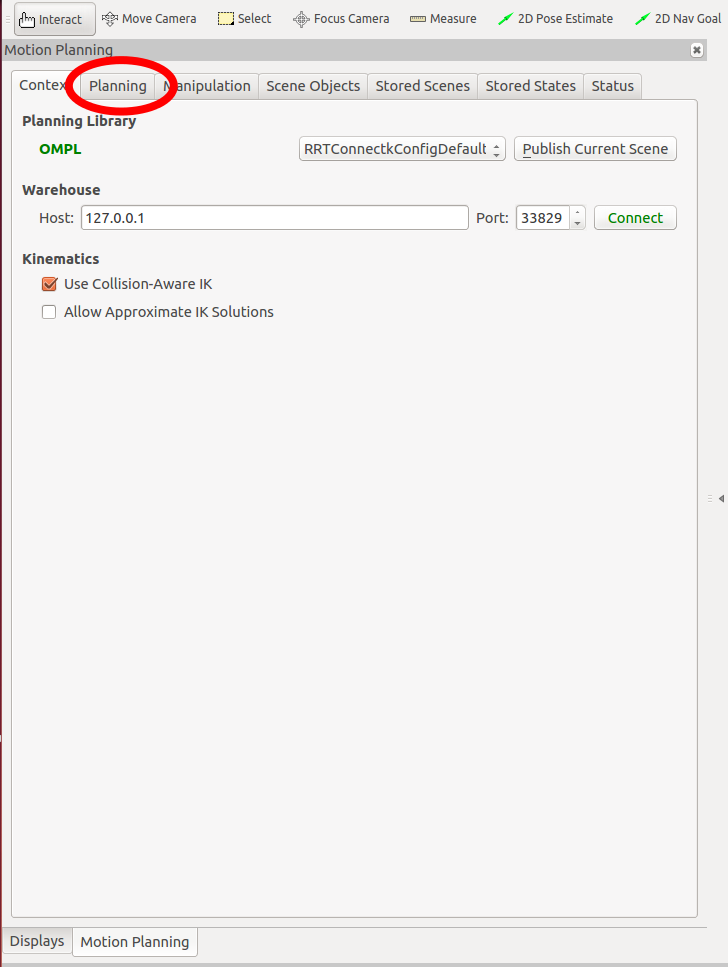
\includegraphics[scale=0.23]{images/motion_planning/gui_moving_procedure_2.png}
\centering
\caption{Clicking on \emph{motion planning}, then \emph{planning}.}
\label{fig:gui_procedure_1}
\end{figure}



\begin{figure}
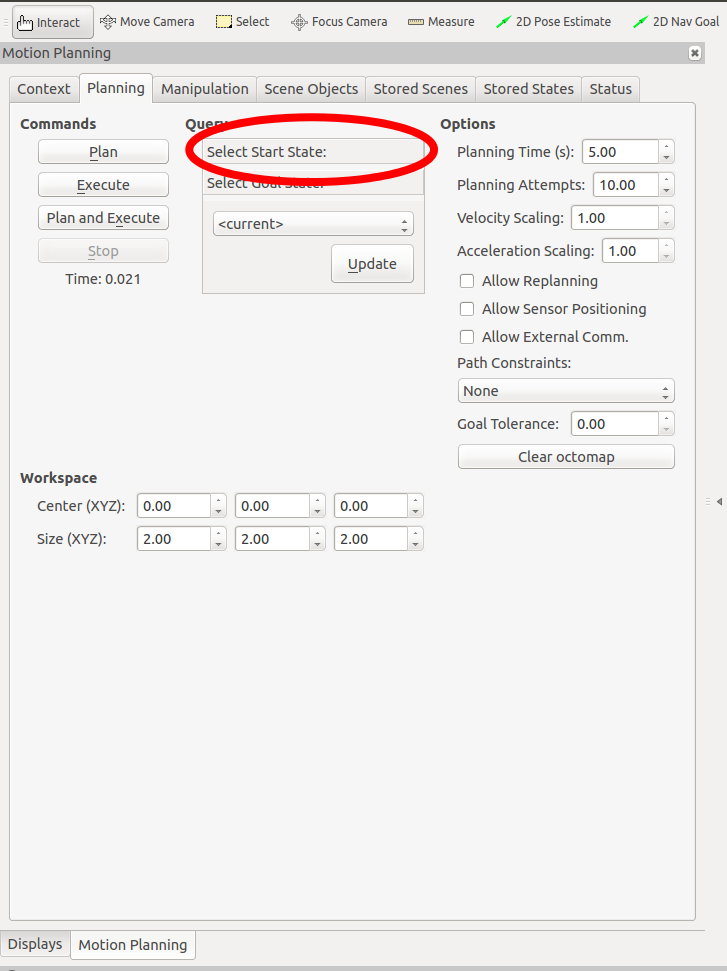
\includegraphics[scale=0.23]{images/motion_planning/gui_moving_procedure_3.png}
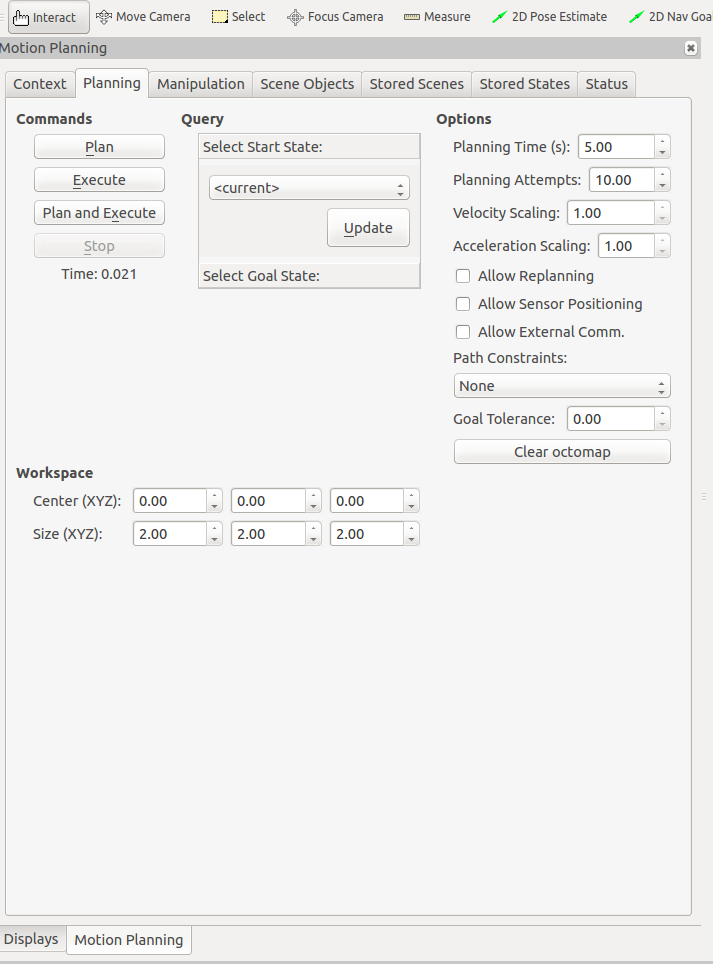
\includegraphics[scale=0.23]{images/motion_planning/gui_moving_procedure_4.png}
\centering
\caption{Clicking on \emph{select start state} and then the \emph{update} button.}
\label{fig:gui_procedure_2}
\end{figure}

\begin{figure}
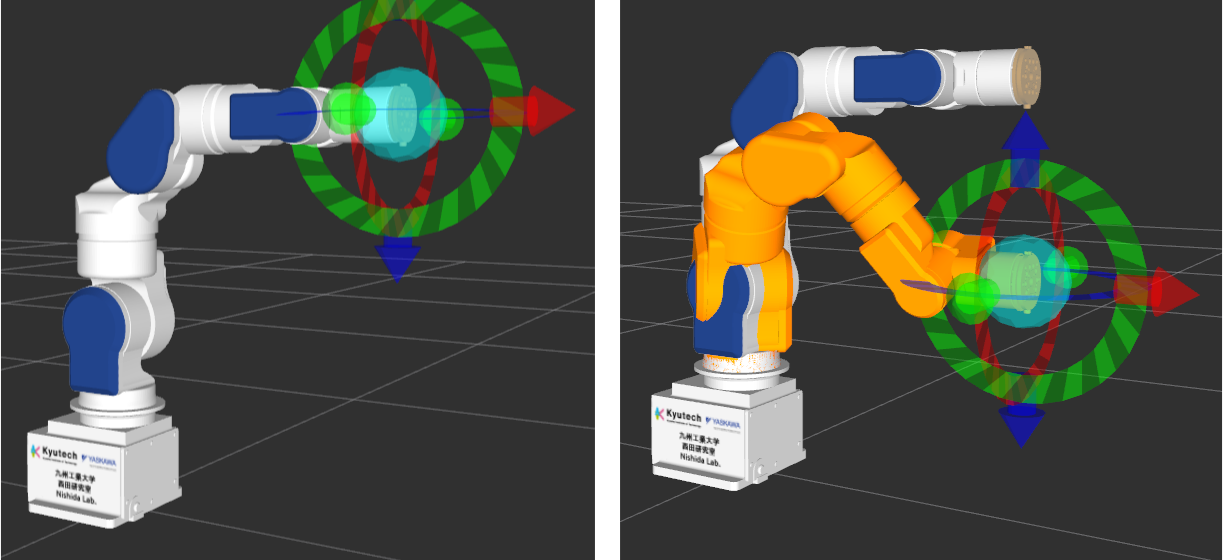
\includegraphics[scale=0.27]{images/motion_planning/gui_end_effector.png}
\centering
\caption{Changing the goal position by moving the end effector ball through the GUI.}
\label{fig:gui_end_effector}
\end{figure}

\section{Simple script}

In this section we review the script we used during chapter 2 to plan a motion between the home position to a specific position. We will describe the different parts of the code and in the following section we will build on this simple script. The script we used is the following one.

\lstinputlisting[language=c++,caption=moving.cpp]{code_files/motion_planning/moving.cpp}

The first important line is the creation of the object \emph{group}. Moveit will do the interface between the motion planners and the robot but it needs to be initialized to know what robot (or what part of the robot) to work on. In our case the whole parts of the robot will be used and it has been named \emph{arm} during the moveit initialization procedure, that is why we put it as an argument. Then we need to define the start and goal position for our planning problem. In this simple script we define the start position as the current position of the robot. Hence we need to get the current position of the robot with the method \emph{getCurrentState} of our object \emph{group}. For the goal position, we decided to define by ourself the exact position of all the joints of the robot and input it as the goal. To do it we first define a map data structure which will associate for each string (the name of the joint) a double (the joint value). The robot is a 7 degrees of freedom robot so there are 7 joints to give values to. Each joint has a name, you can see in figure \ref{fig:sia5_joints_name} their position with their name. The \emph{setJointValueTarget} method of the object \emph{group} is then the method to call to input the goal position from the previously created map. Eventually we need to call the \emph{plan} method from the \emph{group} object, but this method requires a \emph{Plan} object as argument to store the solution (or nothing if no plan is found). It should be noted that the plan method returns a boolean indicating if a solution has been found or not.

So this script was a really simple one to show the basis of a planning with the moveit library. In the following sections we will show how to add some obstacles in the environment, to change the motion planner and how to do a lot of planning.


\section{Moving to a pose}

Instead of specifying all the joint values it can be useful to just ask the end-effector to be at a defined pose (position and orientation). It is simple to do with moveit but be careful as your specified pose may not be possible to reach by the robot end-effector. The following code is the entire code to plan a motion to a pose goal.

\lstinputlisting[language=c++,caption=moving.cpp]{code_files/motion_planning/moving_to_pose.cpp}

You can see that the only part that changed was the goal state definition compared to the simple script. We first create a \emph{Pose} object and then set its attributes. Finally we inform moveit by using the \emph{setPoseTarget} method.


\section{Changing motion planner}

If you want to use an other motion planner than the default one you can do it quite easily ! If the motion planner you want to use is inside OMPL then you simply need to use the method \emph{setPlannerId} with the name of the planner for attribute. For instance, if you want to use the TRRT motion planner just add the following line.


\begin{lstlisting}[language=c++]
group.setPlannerId("TRRTkConfigDefault");
\end{lstlisting}

Here is the list of planner's name you can use :
\begin{itemize}
\item SBLkConfigDefault
\item ESTkConfigDefault
\item LBKPIECEkConfigDefault
\item BKPIECEkConfigDefault
\item KPIECEkConfigDefault
\item RRTkConfigDefault
\item RRTConnectkConfigDefault
\item RRTstarkConfigDefault
\item TRRTkConfigDefault
\item PRMkConfigDefault
\item PRMstarkConfigDefault
\end{itemize}

If you want to use the STOMP planner you cannot use the method \emph{setPlannerId}, instead you will need to modify the launch file. You will need to put \emph{stomp} inside the \emph{planning\_config} argument, \emph{false} for the \emph{use\_ompl} argument and \emph{true} for the \emph{use\_stomp} argument like the following. 



\begin{lstlisting}
<!-- Choose planner [ompl|chomp|stomp] -->
<arg name="planning_config" default="stomp"/>
<!-- If you choose ompl, "use_ompl" is true. -->
<arg name="use_ompl" default="true"/>
<!-- If you choose stomp, "use_stomp" is true. -->
<arg name="use_stomp" default="false"/>
\end{lstlisting}


\section{Adding an obstacle}
\subsection{A simple box}

The previous scripts we have shown are a bit boring without any obstacle. In this section we will explain how to add an obstacle which will be visible in Rviz. First you will need to include the \emph{planning\_scene\_interface.h} file and create a \emph{PlanningSceneInterface} object. This object will be used to add obstacle in the moveit environment. Then you will need to create a vector which will contain all the obstacles you want to add. An obstacle is a \emph{CollisionObject} object, it will need a unique to be identified. In this simple example we choose to add a box as obstacle, you should then first define its dimensions. When the shape of the obstacle has been defined (in this case a box) you will need to define its pose in the environment. In this example we only choose its $(x,y,z)$ coordinates but you can also choose its orientation. Once it has been done you can simply use the \emph{push\_back} method of the obstacle to add its primitive and pose information. Finally you should add the obstacle to the vector previously created and update the \emph{planning\_scene.
}
The following code illustrate all of this. Note that the goal position has been changed to show that the robot needs to avoid the newly add obstacle.


\lstinputlisting[language=c++,caption=moving.cpp]{code_files/motion_planning/add_obstacle.cpp}


\subsection{Other primitives}


\chapter{Real robot}

In this chapter we will learn how to manipulate the real robot instead of only the simulation. Remember that using the robot could be dangerous for you and the other lab members ! Besides, you need to be careful and prevent it to make damage (to the cable or to its surroundings).

\section{Connecting to the robot}

\section{Moving the robot}


\section{Kinect}

In this section we will learn how to use the Kinect and create script to gather the data they collect in real time.
\end{document}





